\section{Exploración Inicial} \label{chapt:initial_exploration}

El objetivo de esta exploración es escoger el valor del tamaño de población. Primero se varía la dimensión
del cromosoma y la población se mantiene fija a 100, para tener una primera idea del comportamiento del algoritmo. 
Se ejecutará el algoritmo 15 veces por cada dimensión del cromosoma, y se cogerá el que tenga mejor valor de fitness para 
la comparación. Los resultados de esta primera exploración se encuentran en la Tabla \ref{tab:fitness_variation}. 

\begin{table}[]
    \centering
    \begin{tabular}{|c|c|c|c|c|c|}
        \hline
        \textbf{Config.} & \multicolumn{1}{l|}{\textbf{DIM}} & \textbf{\begin{tabular}[c]{@{}c@{}}Mediana \\ mejor valor \\ de fitness\end{tabular}} & \textbf{\begin{tabular}[c]{@{}c@{}}Mediana \\ \# ejecuciones \\ de f\end{tabular}} & \textbf{\begin{tabular}[c]{@{}c@{}}$\sigma$\\ mejor valor\\ de fitness\end{tabular}} & \textbf{\begin{tabular}[c]{@{}c@{}}$\sigma$\\ \# ejecuciones \\ de f\end{tabular}} \\ \hline
        1 [\ref{subsect:config_file_1}]                & 2                                 & -73.99                                                                                & 2620.0                                                                             & 2.56                                                                          & 194.18                                                                      \\ \hline
        2 [\ref{subsect:config_file_2}]                & 3                                 & -65.27                                                                                & 2760.0                                                                             & 7.30                                                                          & 123.72                                                                      \\ \hline
        3 [\ref{subsect:config_file_3}]                & 5                                 & -49.48                                                                                & 2900.0                                                                             & 10.94                                                                         & 221.15                                                                      \\ \hline
        4 [\ref{subsect:config_file_4}]                & 10                                & -11.50                                                                                & 7033.0                                                                             & 18.71                                                                         & 1707.48                                                                     \\ \hline
        5 [\ref{subsect:config_file_5}]                & 20                                & 96.16                                                                                 & 6733.0                                                                             & 22.90                                                                         & 1530.60                                                                     \\ \hline
        6 [\ref{subsect:config_file_6}]                & 40                                & 468.68                                                                                & 7902.0                                                                             & 48.57                                                                         & 1039.32                                                                     \\ \hline
    \end{tabular}
    \caption{Resultados de la exploración inicial para diferentes dimensiones del cromosoma y tamaño de población 100}
    \label{tab:fitness_variation}
\end{table}

\begin{figure}[]
	\centering	
	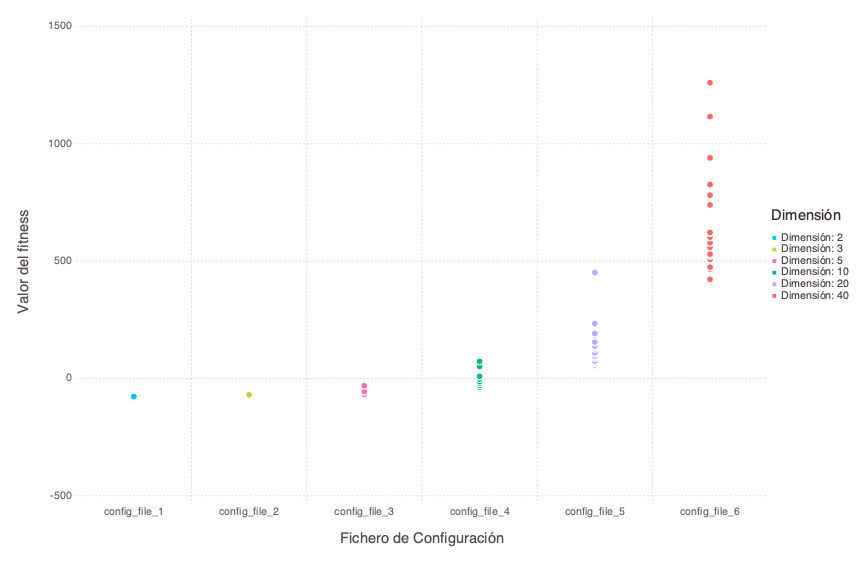
\includegraphics[scale=0.4]{../data/Plots/config_file_1-6_Rastrigin_box_plots.png}
	\caption{ Valores de la función Rastrigin de la ejecución con mejor valor de fitness para cada fichero de configuración }
    \label{fig:box_plots}
\end{figure}

Para un tamaño de población 100 aparentemente la mejor dimensión es la 2, ya que es la que tiene la mediana de mejores valores de fitness con el
menor número de ejecuciones de f. Sin embargo, mirando la Figura \ref{fig:box_plots} comprobamos
que la configuración 1 apenas ha explorado el espacio, entonces ha alcanzado un óptimo local, al igual que de la 2 y la 3. Para
futuras explotaciones descartaremos estas configuraciones, ya que no aportan apenas información sobre el comportamiento del algoritmo, además
de quedar estancadas en óptimos locales en las primeras generaciones. Con la información extraída de estos experimentos no se puede concluir 
qué valores escoger para el tamaño de población ni para la dimensión del cromosoma. En las siguientes secciones se le dará un enfoque diferente.
Para las siguientes exploraciones se usará como base el fichero de configuración 4 \ref{subsect:config_file_4} , ya que quitando los descartados, es el que tiene mejor mediana 
con una dispersión más alta.
